\documentclass[aspectratio=169]{beamer}
\usetheme{FLUKA}
\usepackage[utf8]{inputenc}
\usepackage[english]{babel}
\usepackage[T1]{fontenc}

%%% Feel free to remove these lines - they are needed for these slides only
\usepackage{lipsum}
\usepackage{pgfplots}
\pgfmathdeclarefunction{gauss}{2}{
  \pgfmathparse{1/(#2*sqrt(2*pi))*exp(-((x-#1)^2)/(2*#2^2))}%
}
\usetikzlibrary{calc,positioning}
%%%

\title{Your lecture title}
\location{Lanzhou}{2024}
\author{Your Name}

\AtBeginSection[]{%
  \begin{frame}<beamer>{Outline}
    \tableofcontents[currentsection]
  \end{frame}
}

\begin{document}

\begin{frame}[plain]
\maketitle
\end{frame}

\begin{frame}{Outline}
\tableofcontents
\end{frame}

\section{Fonts}
\begin{frame}{\secname}
  \framesubtitle<1>{Titlepage: title}
  \framesubtitle<2>{Titlepage: location and date}
  \framesubtitle<3>{Normal text}
  \framesubtitle<4>{Text in footer}
  \framesubtitle<5>{Header: slide title}
  \framesubtitle<6>{Header: slide subtitle}
  \framesubtitle<7>{Block title}
  \framesubtitle<8>{Block text}
  \framesubtitle<9>{Itemize/enumerate body}
  \framesubtitle<10>{Itemize/enumerate subbody}
  \framesubtitle<11>{Itemize/enumerate subsubbody}
  \foreach \aaa [count=\i from 1] in {title, date, normal text, author in foot, frametitle, framesubtitle, block title, block text, itemize/enumerate body, itemize/enumerate subbody, itemize/enumerate subsubbody} {
    \only<\i>{
      \usebeamerfont{\aaa}
      \showfont
    }
  }
\end{frame}


\section{Colours}

\begin{frame}{\secname}
  \centering
  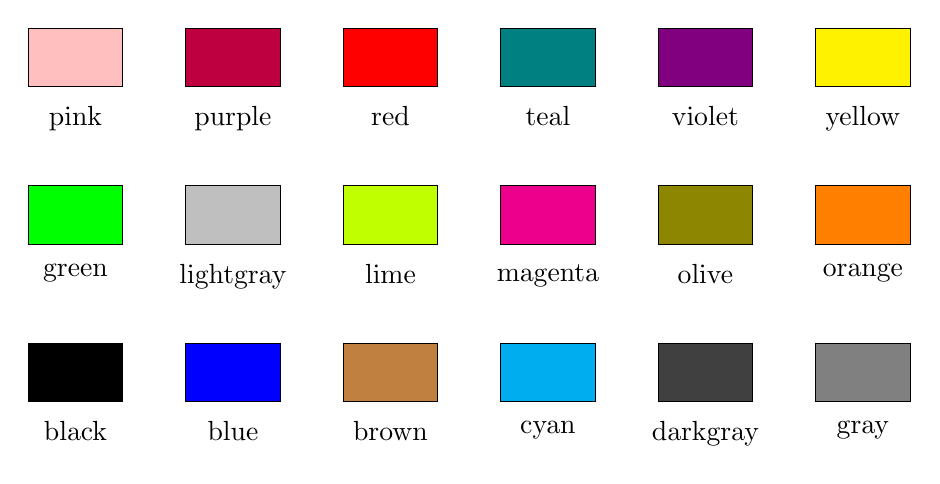
\begin{tikzpicture}
    \def \nColumns {6};
    \def \baseWidth {0.6cm};
    \def \baseHeight {0.37267081cm};

    \foreach \color [count=\i from 0] in {black, blue, brown, cyan, darkgray, gray,
      green, lightgray, lime, magenta, olive,
      orange, pink, purple, red, teal, violet,
      yellow} {
      \coordinate (center_\color)
      at ({2*mod(\i, \nColumns)}, {2*div(\i, \nColumns)});
      \coordinate (rectangle_bottom_\color)
      at ($(center_\color) - (\baseWidth, \baseHeight)$);
      \coordinate (rectangle_top_\color)
      at ($(center_\color) + (\baseWidth, \baseHeight)$);

      \draw[fill=\color, black] (rectangle_bottom_\color) rectangle (rectangle_top_\color);
      \node[below=0.5cm of center_\color] {\color};
    }
  \end{tikzpicture}
\end{frame}

 \section{Math}
 \begin{frame}{\secname}{Equation}
   \centering
   \Huge
   $$
   u(\rho,t) = J_0(k\rho) \cos(2\pi f t)
   $$
 \end{frame}

 \begin{frame}{\secname}{Matrix}
   \centering
   \Huge
   $$
   \mu = \left(
     \begin{array}{ccc}
       \mu_{1} & -jk & 0 \\
       jk & \mu_{1} & 0 \\
       0 & 0 & 1
     \end{array}
   \right)
   $$
 \end{frame}

 \section{Blocks}
 \begin{frame}{\secname}
   \only<1>{
     \framesubtitle{Block}
     \begin{block}{Block title}
       \lipsum[4]
     \end{block}
   }
   \only<2>{
     \framesubtitle{Exampleblock}
     \begin{exampleblock}{Block title}
       \lipsum[4]
     \end{exampleblock}
   }
   \only<3>{
     \framesubtitle{Alertblock}
     \begin{alertblock}{Block title}
       \lipsum[4]
     \end{alertblock}

     Quisque ullamcorper \alert{placerat} ipsum.
   }
 \end{frame}

\section{Examples}
 \begin{frame}{\secname}
   \only<1>{
     \framesubtitle{Enumerate}
     \begin{enumerate}
     \item \lipsum[1][1] %\lipsum[2][1]
     \item \lipsum[1][2] \lipsum[2][2]
     \item \lipsum[1][3] \lipsum[2][3]
     \end{enumerate}
   }
   \only<2>{
     \framesubtitle{Itemize}
     \begin{itemize}
     \item \lipsum[1][1] %\lipsum[2][1]
     \item \lipsum[1][2] \lipsum[2][2]
     \item \lipsum[1][3] \lipsum[2][3]
     \end{itemize}
   }
   \only<3>{
     \framesubtitle{Table}
     \centering
     \begin{tabular}{ccc}
       \toprule
        $A$ & $B$ & $A\mathbin{\oplus}B$ \\
       \midrule
       0 & 0 & 0 \\
       0 & 1 & 1 \\
       1 & 0 & 1 \\
       1 & 1 & 0 \\
       \bottomrule
      \end{tabular}
   }
   \only<4>{
     \framesubtitle{TikZ picture}
     \centering
     \begin{tikzpicture}
       \begin{axis}[
           height=0.7\textheight,
           width=0.8\linewidth,
           xlabel = {x {[\si{\cm}]}},
           ylabel = {y {[\si{\cm}]}},
           title = {Title},
           view={0}{90},
           colormap/hot,
           colorbar sampled,
           colorbar style={
             title = {Palette title},
             ylabel = {Value {[arb. units]}},
             samples=8,
           },
         ]
	\addplot3[surf] {x*y};
	\end{axis}
     \end{tikzpicture}
   }
   \only<5>{
     \framesubtitle{External graphics}
     \begin{block}{Heavy ion incident onto ATIC spectrometer}
       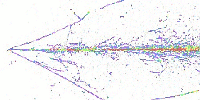
\includegraphics[width=0.49\linewidth]{figs/g1-soft.png} \hfill
       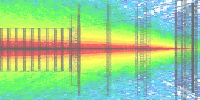
\includegraphics[width=0.49\linewidth]{figs/g5-soft.png}

       \hfill\copyr{http://www.fluka.org}{Toni Empl}
     \end{block}
   }
 \end{frame}

 \section{Bibliography}
 \begin{frame}{\secname}
   \begin{thebibliography}{3}
     \beamertemplatearticlebibitems
   \bibitem{Tantau2010}
     Till Tantau, Joseph Wright, Vedran Mileti\'c
     \newblock The BEAMER class User Guide
     \newblock \href{http://bitbucket.org/rivanvx/beamer}{http://bitbucket.org/rivanvx/beamer}
     \newblock 2010

     \beamertemplatebookbibitems
   \bibitem{Book}
     Book author
     \newblock{Book title}
     \newblock{Year}
   \end{thebibliography}
 \end{frame}

 \finalpage
\end{document}
